
%begin{comment}
%:Title: Work breakdown structures aka WBS diagrams
%:Tags: Charts;Diagrams;Trees
%:Author: Gonzalo Medina
%:Slug: work-breakdown-structure

%A work breakdown structure (WBS) diagram, is for decomposing a task into smaller parts, which helps organizing and performing. This example diagram shows possible tasks for designing a TikZ diagram. The basis is a tree, nodes were addes below its child nodes. It was originally posted by Gonzalo Medina as TeX.SE (http://tex.stackexchange.com/q/81809/213), modified by Stefan Kottwitz.
%\end{comment}
\usetikzlibrary{arrows,shapes,positioning,shadows,trees}

\tikzset{
  basic/.style  = {draw, text width=3cm, drop shadow, font=\sffamily, rectangle},
  root/.style   = {basic, rounded corners=2pt, thin, align=center,
                   fill=blue!30},
  level 2/.style = {basic, rounded corners=6pt, thin,align=center, fill=gray!30,
                   text width=8em},
  level 3/.style = {basic, thin, align=left, fill=brown!60, text width=6.5em, scale = 0.9}
}

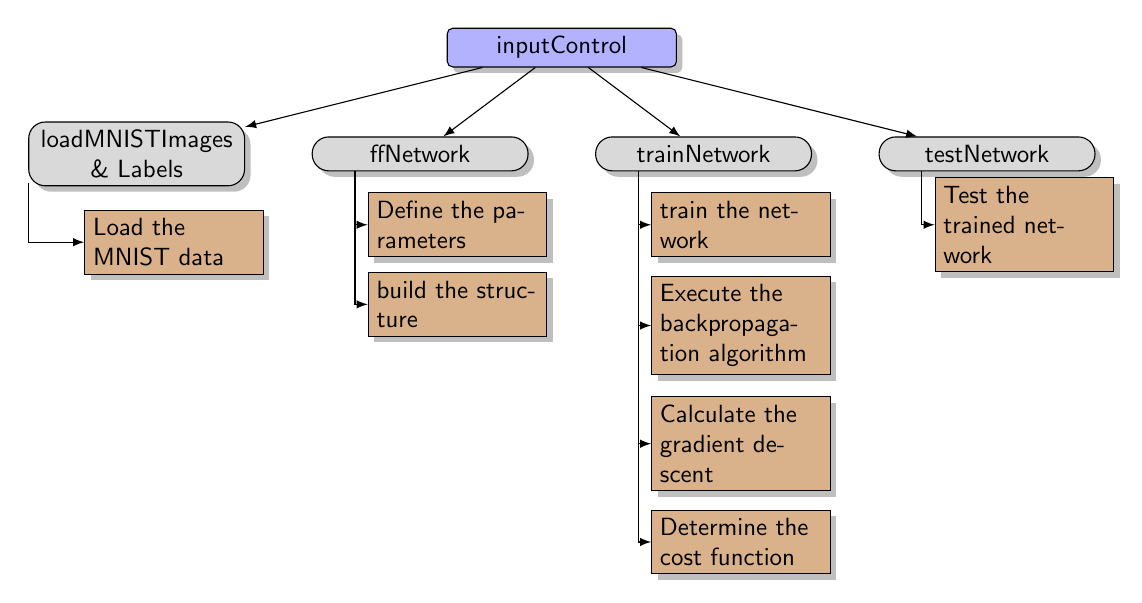
\begin{tikzpicture}[
  level 1/.style={sibling distance=40mm},
  edge from parent/.style={->,draw},
  >=latex,
  scale= 0.9
  ,every node/.style={scale= 0.9}]

% root of the the initial tree, level 1
\node[root] {inputControl}
% The first level, as children of the initial tree
  child {node[level 2] (c1) {loadMNISTImages \& Labels}}
  child {node[level 2] (c2) {ffNetwork}}
  child {node[level 2] (c3) {trainNetwork}}
  child {node[level 2] (c4) {testNetwork}};

% The second level, relatively positioned nodes
\begin{scope}[every node/.style={level 3}]
\node [below of = c1, xshift=15pt, yshift = - 7pt] (c11) {Load the MNIST data};

\node [below of = c2, xshift=15pt] (c21) {Define the parameters};
\node [below of = c21, yshift = -3.5pt] (c22) {build the structure};

\node [below of = c3, xshift=15pt] (c31) {train the network};
\node [below of = c31, yshift = -12pt] (c32) {Execute the backpropagation algorithm};
\node [below of = c32, yshift = -19pt] (c33) {Calculate the gradient descent};
\node [below of = c33, yshift = -11pt] (c34) {Determine the cost function};


\node [below of = c4, xshift=15pt] (c41) {Test the trained network};

\end{scope}

% lines from each level 1 node to every one of its "children"
\foreach \value in {1}
  \draw[->] (c1.195) |- (c1\value.west);

\foreach \value in {1,2}
  \draw[->] (c2.195) |- (c2\value.west);

\foreach \value in {1,2,3,4}
  \draw[->] (c3.195) |- (c3\value.west);
  
\foreach \value in {1}
  \draw[->] (c4.195) |- (c4\value.west);
  
  
  
\end{tikzpicture}